\section{EXPERIMENT AND EVALUATION}
The experiment utilized the Meta Quest 3 as the VR headset to provide users with visual information, while VR twins served as the interaction method to deliver haptic feedback. The program's interaction logic and visualization scenarios were implemented using Unity 2021.3.32f1c1. The VR twins employed gesture-tracking technology to visualize the user's physical hand as a virtual hand for interaction, with real-time data updates and synchronization achieved through sensing technology. Gesture tracking was implemented using the Meta XR All-in-One SDK (v63). The system framework is illustrated in Figure \ref{fig:system-framework-flowchart}.

\begin{figure*}[t]
  \centering
  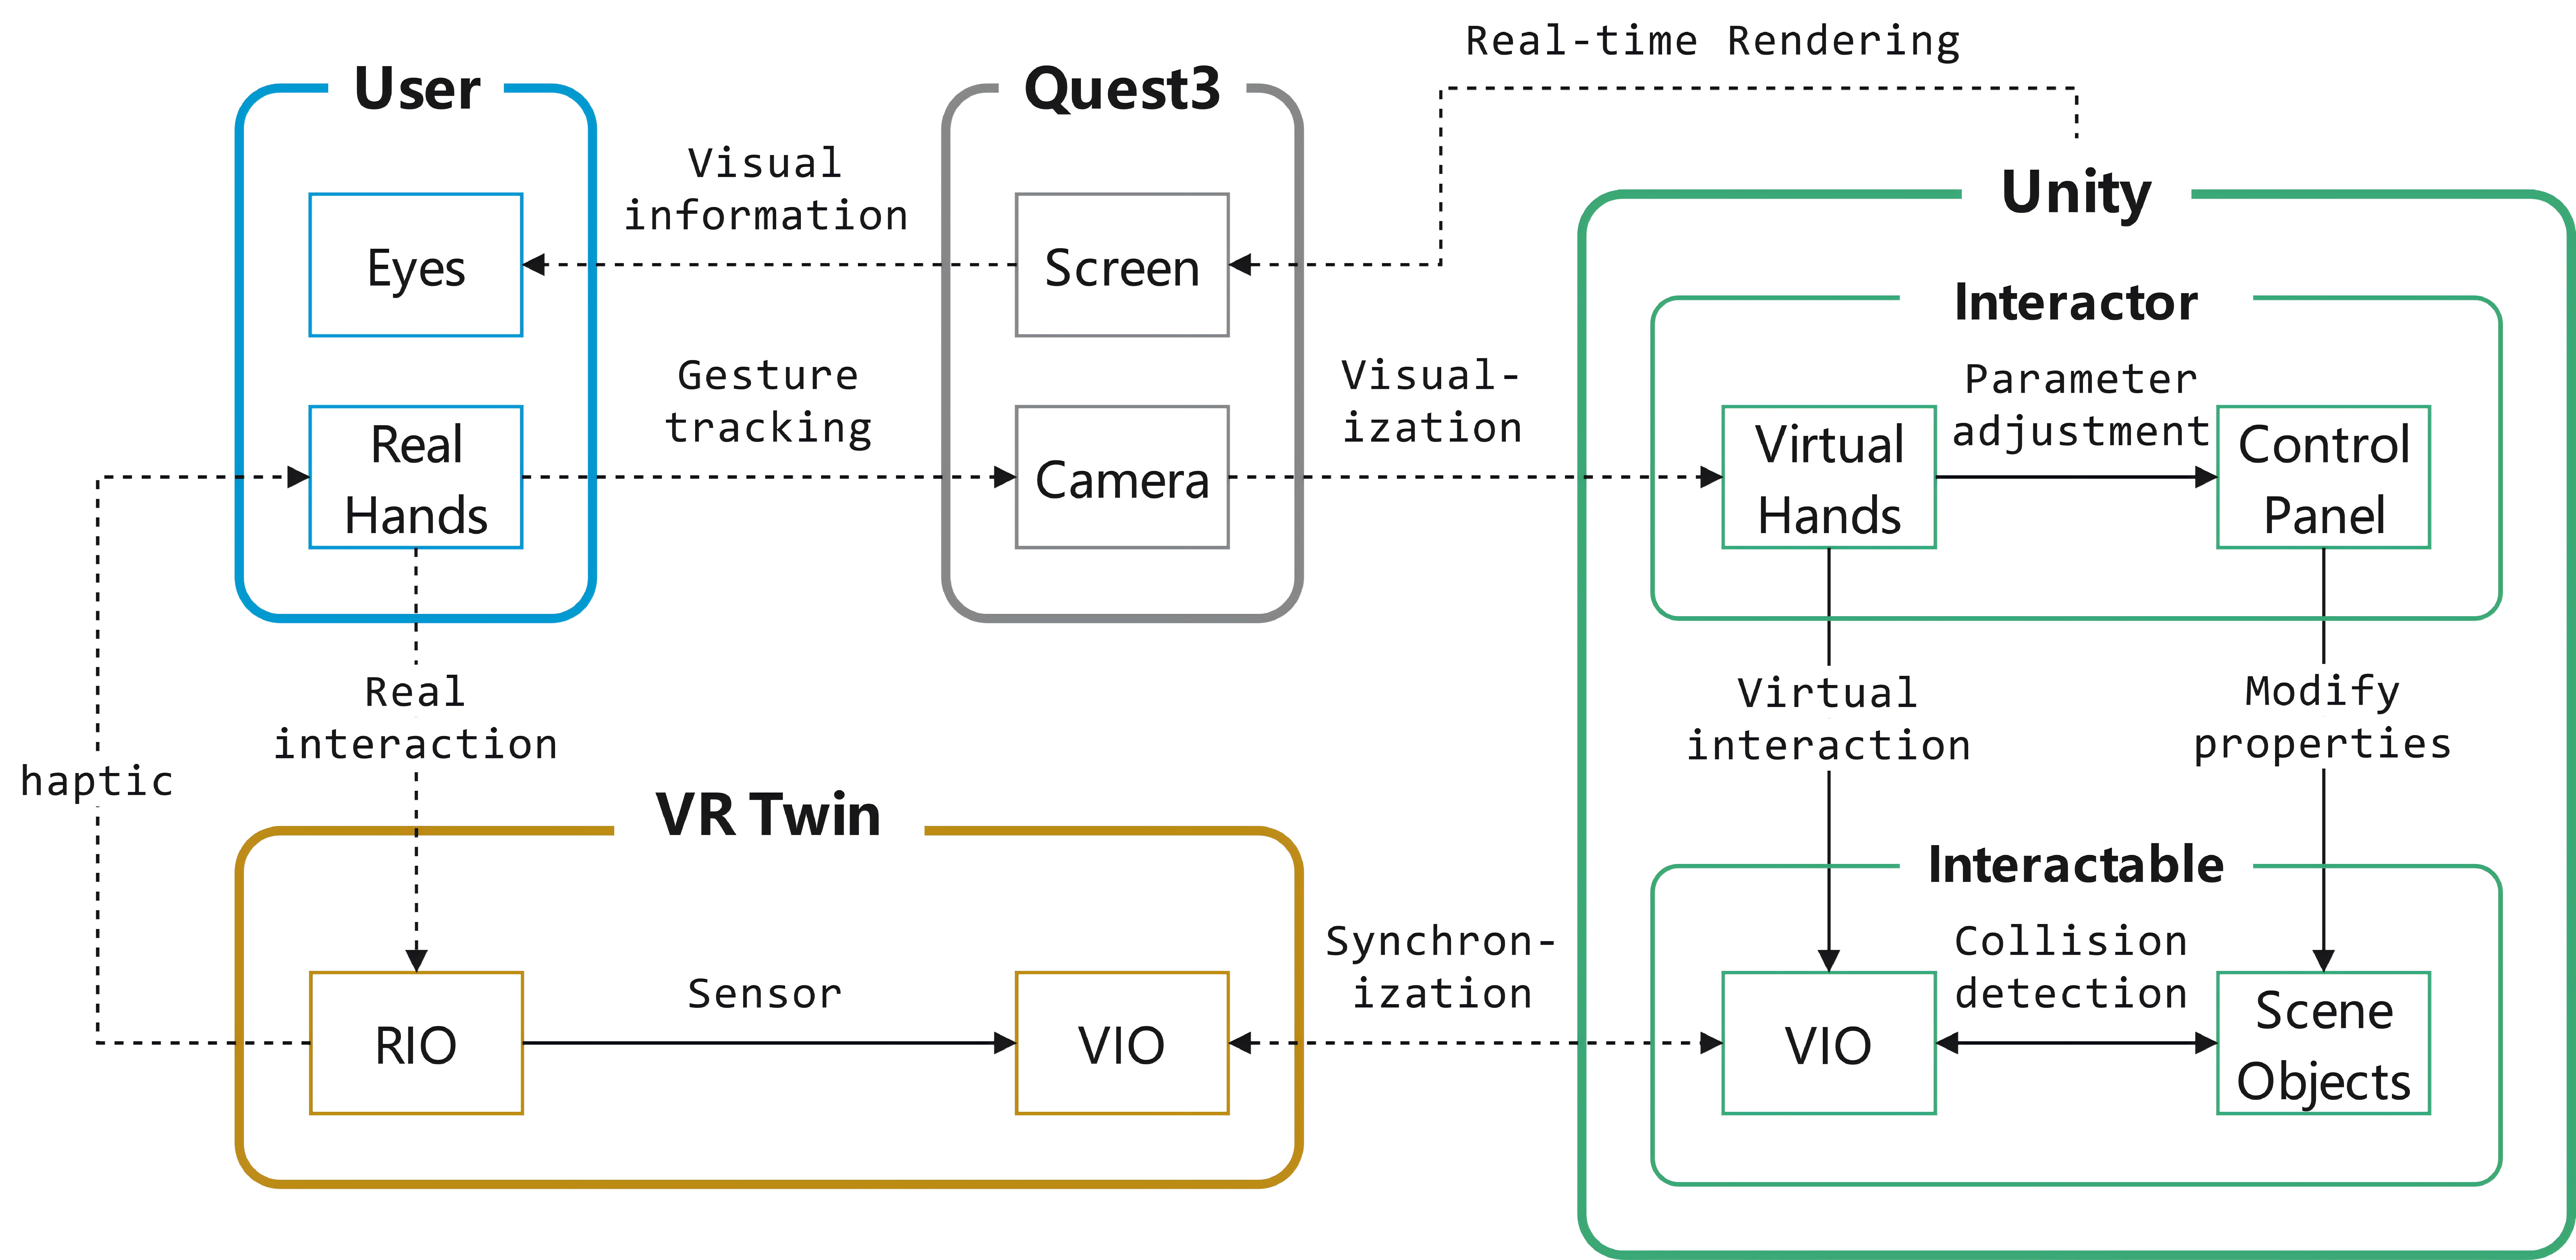
\includegraphics[width=1\textwidth]{image/system-framework-flowchart.pdf}
  \caption{System framework flowchart.}
  \label{fig:system-framework-flowchart}
\end{figure*}

\subsection{Evaluation Methods}
This study compares VRTI (with realistic haptic feedback, experimental group) and GI (without realistic haptic feedback, control group). The only difference between the two interaction methods is the presence or absence of real haptic feedback. Through a comparative experiment, the study investigates the impact of real haptic feedback on students' physics experiments in terms of cognitive load, learning motivation, immersion, and learning outcomes.

\subsubsection{User Experience}
\begin{enumerate}
  \item {\texttt{Cognitive Load}}: Cognitive load is measured using the Klepsch Scale \cite{klepsch2017development}, which assesses three dimensions: intrinsic cognitive load, extraneous cognitive load, and germane cognitive load. In haptic feedback tasks, multimodal interactions between haptic and visual/auditory information may reduce extraneous cognitive load through "attention guidance" but could also increase germane cognitive load due to "cross-modal switching."

  \item {\texttt{Learning Motivation}}: Learning motivation is measured using the Keller Scale \cite{keller1983motivational}, based on the ARCS model of motivation. It evaluates four dimensions: Attention, Relevance, Confidence, and Satisfaction, assessing learners' internal drive to engage in and complete learning tasks. When exposed to new technologies like haptic feedback, learners' intrinsic motivation (e.g., curiosity and desire to explore) or extrinsic motivation (e.g., rewards for task completion) may significantly influence their engagement and learning effectiveness. Higher motivation increases the likelihood of students persisting through challenges, thereby leveraging haptic feedback technology for effective learning.

  \item {\texttt{Immersion}}: Immersion is measured using the Schubert Scale \cite{schubert2001experience}, focusing on the sense of presence in the virtual environment. It comprehensively evaluates students' immersion and sense of control through three dimensions: spatial presence, involvement, and perceived realism of the virtual environment.
\end{enumerate}

All scales were translated and localized to ensure their suitability for the cultural and educational context of this experiment.

\subsubsection{Physics Knowledge}
The physics knowledge test was provided by Professor XXX
% Xiang Hua 
and his team from the Physics Department of XXX
% Beijing Normal 
University. It consists of a pre-test and a post-test.

\begin{enumerate}
  \item {\texttt{Pre-test}}: Includes 16 items, with 6 focusing on basic physics knowledge to assess students' foundational understanding and 10 related to the experiment for comparison with the post-test results.

  \item {\texttt{Post-test}}: Includes 16 items, with 10 being similar to the pre-test's experiment-related questions (with changes in narrative and data) and 6 being more challenging comprehensive application questions to evaluate students' critical thinking and ability to synthesize knowledge.
\end{enumerate}

Both tests include an "I don't know" option to reduce guessing tendencies and obtain more accurate assessment data.

\subsubsection{Semi-Structured Interviews}
After the user experiment, semi-structured interviews were conducted to explore participants' experiences with VRTI and immersive learning, with follow-up questions to delve deeper. Examples include:

\begin{enumerate}
  \item "What is your overall impression of VRTI?"
  
  \item "What do you think are the differences between VRTI and GI?"
  
  \item "You mentioned 'immersion.' Could you provide an example?"
\end{enumerate}

The interviews aimed to capture personalized perspectives and in-depth insights while ensuring data completeness. Face-to-face interviews were conducted in a private, distraction-free environment, with recordings and notes taken after obtaining participants' consent.

\subsection{Evaluation Process}
\subsubsection{Participants}
A total of 64 high school sophomores from XXX
% Beijing Jingshan 
School were recruited for the experiment. All participants had previously studied the relevant foundational physics knowledge in class. The students were randomly and evenly divided into two groups:

\begin{enumerate}
  \item Experimental Group (N=32): used VRTI.

  \item Control Group (N=32): used GI.
\end{enumerate}

\subsubsection{Experimental Procedure}
To ensure the validity of the results, all participants received a unified experimental introduction and operational guidance before starting the experiment (Figure \ref{fig:experimental-procedure}). The procedure consisted of the following four steps:

\begin{enumerate}
\item {\texttt{Pre-test}}: Students independently completed a pre-test questionnaire, which took approximately 10 minutes.

\item {\texttt{Experimental Introduction}}: Students watched an instructional video to familiarize themselves with the experimental operations and procedures, which took approximately 5 minutes.

\item {\texttt{Experimental Operation}}: Students performed the experiment according to their assigned group, which took approximately 15 minutes.

\item {\texttt{Post-test}}: Students independently completed a post-test questionnaire, which included 30 user experience evaluation items (cognitive load, learning motivation, immersion) and 15 physics knowledge evaluation items, taking approximately 30 minutes.

\begin{figure}
  \begin{subfigure}{0.48\linewidth} % 子图 (a)
    \centering
    \includegraphics[width=\linewidth]{image/experimental-introduction.pdf}
    \caption{} % 子图标题 (a) 的内容
    \label{fig:experimental-introduction}
  \end{subfigure}
  \hfill % 水平填充间隔
  \begin{subfigure}{0.48\linewidth} % 子图 (b)
    \centering
    \includegraphics[width=\linewidth]{image/experimental-operation.pdf}
    \caption{} % 子图标题 (b) 的内容
    \label{fig:experimental-operation}
  \end{subfigure}
  \caption{Experimental procedure demonstration. (\subref{fig:experimental-introduction}) Experimental introduction, (\subref{fig:experimental-operation}) Experimental operation.}
  \label{fig:experimental-procedure}
\end{figure}

\end{enumerate}

Throughout the experiment, group assignments were randomized to ensure balance between the groups. Teaching assistants supervised the entire process to ensure that each participant strictly followed the experimental procedure.

\subsection{Results Analysis}
\begin{figure*}[t]
  \centering
  \begin{subfigure}{0.45\textwidth} % 子图 (a)
    \centering
    \includegraphics[width=\linewidth]{image/pre-test-result.pdf}
    \caption{} % 子图标题 (a) 的内容
    \label{fig:pre-test-result}
  \end{subfigure}
  \hspace{0.05\textwidth} % 水平填充间隔
  \begin{subfigure}{0.45\textwidth} % 子图 (b)
    \centering
    \includegraphics[width=\linewidth]{image/user-experience-result.pdf}
    \caption{} % 子图标题 (b) 的内容
    \label{fig:user-experience-result}
  \end{subfigure}
  \caption{Pre-test and user experience results. (\subref{fig:pre-test-result}) Pre-test result, (\subref{fig:user-experience-result}) User Experience result.}
  \label{fig:pre-test-and-user-experience-result}
\end{figure*}

\begin{figure*}[t]
  \centering
  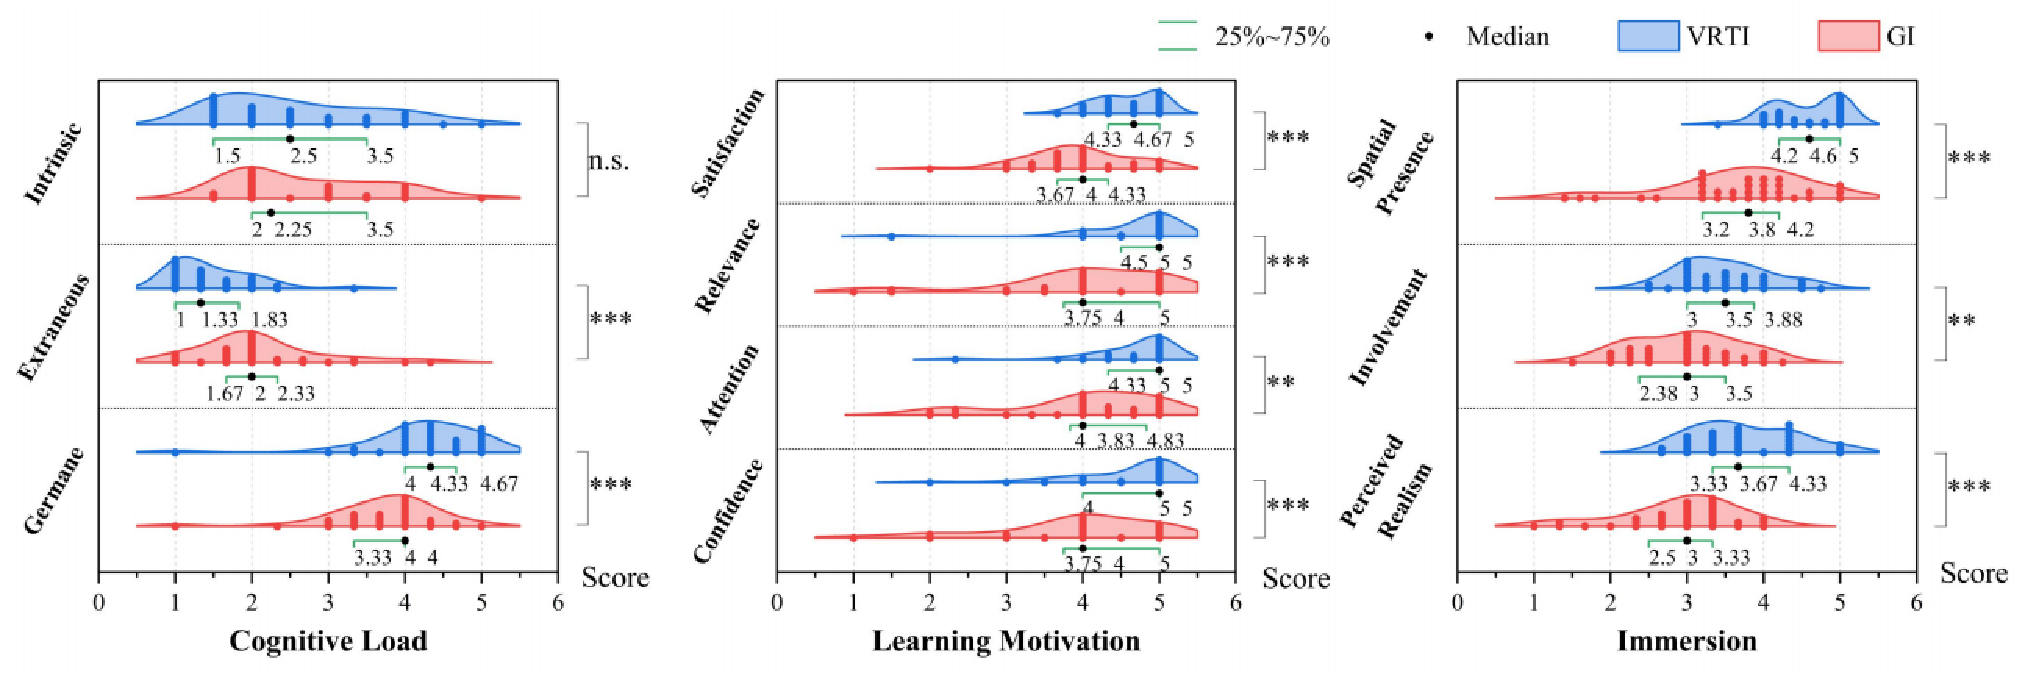
\includegraphics[width=\textwidth]{image/three-user-experience-result.pdf} % 使用\textwidth而非\linewidth
  \caption{Comparison of each user experience between VRTI and GI.}
  \label{fig:three-user-experience-result}
\end{figure*}

According to Shapiro-Wilks tests, only the experiment-related content test results in the experimental group followed a normal distribution, while all other measures violated this assumption. Consequently, the Mann-Whitney U test was employed to analyze between-group differences. Significance levels were denoted as follows: $p \le 0.05$ (*) for significant differences, $p \le 0.01$ (**) for highly significant differences, and $p \le 0.001$ (***) for extremely significant differences. Effect sizes were interpreted as: $|r| \le 0.1$ indicating small effects, $0.1 < |r| \le  0.3$ representing medium effects, and $d > 0.5$ reflecting large effects.

\subsubsection{Prior Analysis}
The pre-test included 6 basic physics concept questions and 10 experiment-related questions, each scored 1 point, totaling 16 points. Figure \ref{fig:pre-test-result} shows the pre-test results for both groups, with bar lengths representing the mean (Mean) and black error bars indicating 1.0 × standard deviation (SD). The Mann-Whitney U Test (M-U Test) results revealed no significant differences between the experimental and control groups in basic physics concepts ($p=0.600$), momentum conservation knowledge ($p=0.984$), or overall scores ($p=0.834$). Therefore, it can be concluded that the two groups had comparable prior physics knowledge.

Figure \ref{fig:user-experience-result} compares the user experience between the experimental and control groups across three dimensions: cognitive load, learning motivation, and immersion.Solid circles above each group represent sample points, with kernel smoothing used to fit curves describing their distribution. Below, Type I boxplots show the 25\% (Q1), 50\% (Q2), and 75\% (Q3) quartiles.

\subsubsection{Cognitive Load}
There was no significant difference in intrinsic cognitive load between the two groups ($Z=-0.720, p=0.472, |r|=0.127$). The extraneous cognitive load in the experimental group was significantly lower than that in the control group ($Z=-3.538, p<0.001, |r|=0.625$), showing a large effect. Conversely, the germane cognitive load in the experimental group was significantly higher ($Z=-3.337, p=0.001, |r|=0.590$), also with a large effect. These results can be explained as follows:

\begin{enumerate}
\item {\texttt{Intrinsic Cognitive Load}}: The addition of realistic haptic feedback does not affect the inherent complexity of the learning task, which aligns with Cognitive Load Theory. Intrinsic cognitive load is related to the essential complexity of the task and is difficult to change significantly through interaction methods.

\item {\texttt{Extraneous Cognitive Load}}: VRTI reduces unnecessary load caused by redundant or distracting information during operations by providing realistic haptic feedback.

\item {\texttt{Germane Cognitive Load}}: Realistic haptic feedback promotes the construction and automation of cognitive structures, enhancing learning and understanding.
\end{enumerate}

\subsubsection{Learning Motivation}
The experimental group showed significant improvements in attention ($Z=-3.382, p=0.001, |r|=0.598$), relevance ($Z=-3.313, p=0.001, |r|=0.586$), confidence ($Z=-3.001, p=0.003, |r|=0.531$), and satisfaction ($Z=-4.127, p<0.001, |r|=0.730$), all with large effects. These results can be explained as follows:

\begin{enumerate}
  \item {\texttt{Attention}}: Realistic haptic feedback in immersive learning environments attracts learners' interest more effectively.

  \item {\texttt{Relevance}}: Customized content design enhances the connection between the learning material and the learners.

  \item {\texttt{Confidence}}: Immediate feedback and interactive experiences provided by VRTI boost learners' confidence.

  \item {\texttt{Satisfaction}}: Realistic haptic feedback provides a sense of achievement during interactions, increasing learners' satisfaction.
\end{enumerate}

\subsubsection{Immersion}
The experimental group showed significant improvements in spatial presence ($Z=-4.524, p<0.001, |r|=0.800$), involvement ($Z=-2.774, p=0.006, |r|=0.490$), and perceived realism ($Z=-4.102, p<0.001, |r|=0.725$), all with large effects. These results can be explained as follows:

\begin{enumerate}
  \item {\texttt{Spatial Presence}}: Realistic haptic feedback significantly enhances learners' sense of spatial presence.

  \item {\texttt{Involvement}}: The well-designed interaction of VR twins significantly increases learners' engagement.

  \item {\texttt{Perceived Realism}}: High-fidelity visual and haptic experiences in VRTI significantly enhance the realism of the learning environment.
\end{enumerate}

\subsubsection{Learning Outcomes}
Figure \ref{fig:improvements-result} presents the comparative results of pre-test and post-test improvements in momentum concept, experimental understanding, and total scores, along with performance on comprehensive application. Both momentum concept and experimental comprehension assessments consisted of 5 test items each, with each item worth 1 point (total 10 points).

The experimental group showed significant improvement in experimental understanding ($Z=-1.967, p=0.05, |r|=0.347$), with a medium effect, but no significant improvement in momentum concept ($Z=-0.354, p=0.724, |r|=0.063$) or overall scores ($Z=-1.714, p=0.087, |r|=0.303$). Additionally, the experimental group performed significantly better in comprehensive application tests ($Z=-2.828, p=0.005, |r|=0.500$), with a large effect. This indicates that VRTI, through realistic haptic feedback, helps learners understand experimental content more intuitively and enhances their comprehensive application abilities. However, mastery of momentum concepts relies more on learners' prior knowledge and abstract thinking skills, which VRTI has limited impact on.

\begin{figure}
  \centering
  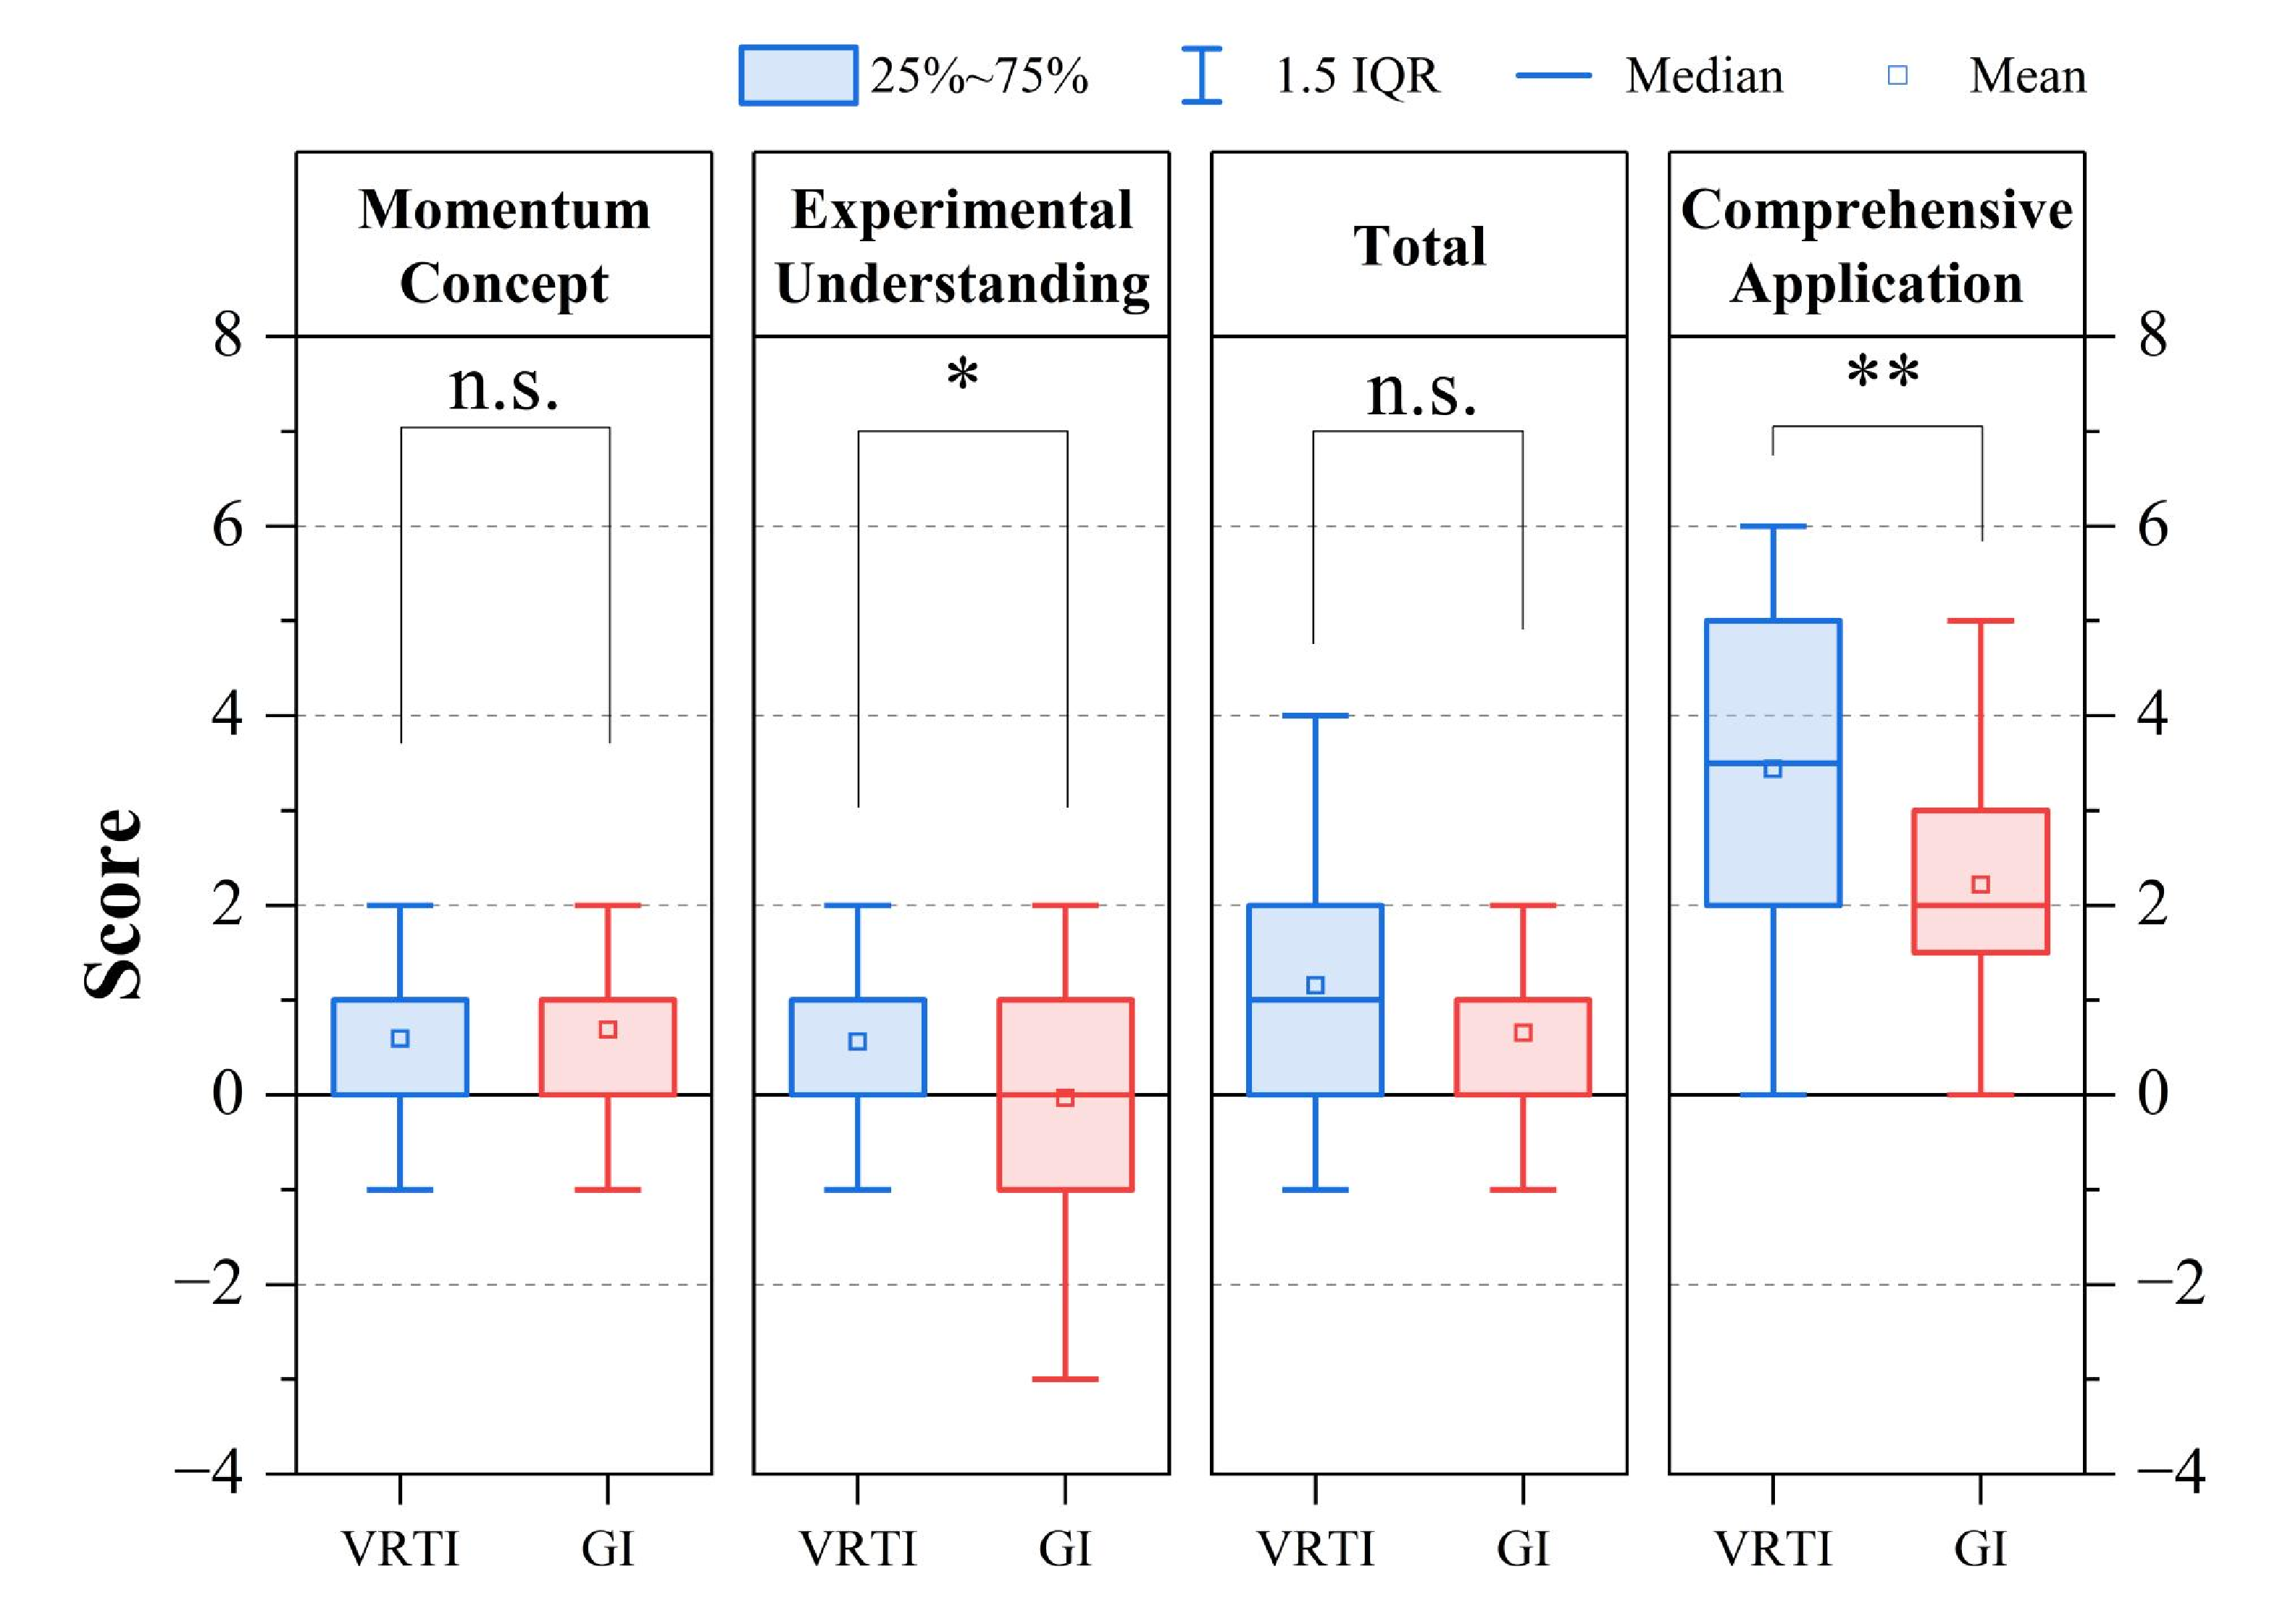
\includegraphics[width=0.8\linewidth]{image/improvements-result.pdf}
  \caption{The comparative results of pre-test and post-test improvements in momentum concept, experimental understanding, and total scores, along with performance on comprehensive application.}
  \label{fig:improvements-result}
\end{figure}

\subsubsection{Interview Results}
After the experiment, semi-structured interviews were conducted with participants to explore their subjective experiences with VRTI and GI. Key findings include:

\begin{enumerate}
  \item {\texttt{Overall Experience}}: Most users gave positive feedback on the haptic feedback, with one user stating, "VRTI allowed me to feel the weight and resistance of objects, making the operation more immersive." However, some users mentioned that prolonged use of GI could lead to arm fatigue: "Keeping my arms suspended for a long time during GI made me feel tired."

  \item {\texttt{Comparison with GI}}: Users generally agreed that the VRTI outperformed GI in terms of haptic feedback and operational intuitiveness. One user noted, "GI offers freedom of movement, but the lack of realistic haptic feedback makes it feel incomplete." Conversely, some users highlighted the flexibility of GI: "GI allows me to adjust hand positions freely, while the VRTI requires fixed positions."

  \item {\texttt{Immersion Experience}}: Users widely acknowledged that the VRTI significantly enhanced their sense of immersion in the virtual environment. One user explained, "When I pulled the spring, I could feel its resistance, which made me feel like I was actually conducting a physical experiment." However, some users reported that the quality of haptic feedback degraded with frequent use: "After multiple experiments, the haptic feedback of the device became less responsive."

  \item {\texttt{Improvement Suggestions}}: Users proposed several suggestions for improving the VRTI. For instance, one user recommended optimizing the support structure of the device to reduce operational fatigue: "If a support frame could be designed to keep the arms from being suspended all the time, the operation would be more comfortable." Additionally, users emphasized the need to enhance the durability of the device: "The haptic feedback of the device diminished after repeated use, and I hope this can be improved in the future."
\end{enumerate}